\chapter{Dataset}\label{chap:dataset}
In questo capitolo tratteremo la generazione del dataset posto alla base del modello che andremo a creare poi nel \autoref{chap:modello}. 
Vederemo prima il dataset originale utilizzato e poi come è stato aumentato tramite l'utilizzo di ulteriori analizzatori statici per migliorarne la precisione delle rilevazioni, andando a ridurre il numero di falsi positivi.
Verrà poi presentato come le rilevazioni degli analizzatori statici sono utilizzate per la associazione fra un \textit{code snippet} e il relativo errore, poi come da quest'ultimo venga ricavato il codice in formato di \textit{ast context vector}.

\section{Dataset originale}
Come detto in precedenza questo dataset non è stato generato partendo da zero ma facendo riferimento al dataset creato da \cite{gelman2019source}. Il dataset consiste di circa 3000 progetti di GitHub, scritti in linguaggi C e \CPP,
 che rispettano due requisiti: hanno una licenza ridistribuibile e hanno almeno 10 stelle.
 Il secondo requisito ci serve per garantire che i progetti all'interno del dataset soddisfino dei requisiti di qualità, infatti come precedenti studi hanno mostrato (come ad esempio \cite{papamichail2016user}) si può utilizzare il numero
 di stelle su GitHub come un \textit{proxy} per la qualità del codice stesso.

Il dataset contiene per ogni progetto una serie di analisi effettuate: l'analisi di Doxygen che estrae le coppie codice-commento e l'analisi di Infer che produce un report di analisi statica degli errori.
Visto l'utilizzo che ne sarebbe stato fatto di questo dataset l'analisi di Doxygen è stata scartata. In \autoref{fig:dir_struct} si può vedere la struttura tipica di uno dei circa 3000 progetti presenti.
\begin{figure}
    \centering
    \scalebox{0.6}{
        \begin{forest}
            for tree={
                font=\ttfamily,
                grow'=0,
                child anchor=west,
                parent anchor=south,
                anchor=west,
                calign=first,
                inner xsep=7pt,
                edge path={
                  \noexpand\path [draw, \forestoption{edge}]
                  (!u.south west) +(7.5pt,0) |- (.child anchor) pic {folder} \forestoption{edge label};
                },
                % style for your file node 
                file/.style={edge path={\noexpand\path [draw, \forestoption{edge}]
                  (!u.south west) +(7.5pt,0) |- (.child anchor) \forestoption{edge label};},
                  inner xsep=2pt,font=\small\ttfamily
                             },
                before typesetting nodes={
                  if n=1
                    {insert before={[,phantom]}}
                    {}
                },
                fit=band,
                before computing xy={l=15pt},
              }  
        [Project-name
          [source
            [Project-name
                [Makefile, file]
                [File1.c, file]
                [File2.c, file]
                [..., file]
                [Folder1]
                [Folder2]
                [...]
            ]
          ]
          [derivatives
            [
                Infer-out
                [bugs.txt, file]
            ]
            ]
            [LICENSE, file]
            [url, file]
        ]
        \end{forest}
    }
    %\includegraphics[scale=0.3]{images/immagineStrutturaDirectoryIniziale.png}
    \caption{La struttura della directory di un progetto del dataset iniziale}
    \label{fig:dir_struct}
\end{figure}

Come si può notare ogni progetto contiene anche un Makefile, elemento fondamentale perché gli analizzatori statici che andremo ad aggiungere spesso richiedono l'esistenza di un Makefile funzionante.

%Figura della struttura delle directory


%\subsection{Dataset originale}
 

%\subsection{Analizzatori utilizzati}

\section{Analizzatori di codice statici}
Un'analizzatore di codice è un programma che prende in input uno o più file e genera un report degli errori, cioè una lista di coppie del tipo $<$Errore, Posizione$>$. Di questi analizzatori ne esistono due macro categorie: statici e dinamici. 
Gli analizzatori statici sono programmi che effettuano controlli solo sul codice a livello testuale e che quindi non eseguono in nessuna maniera il codice. Gli analizzatori dinamici sono invece analizzatori più complessi che effettuano controlli a \textit{run-time}
andando quindi ad'eseguire il codice stesso.

Gli analizzatori non sono però perfetti, infatti nell'insieme degli errori trovati si possono spesso trovare dei falsi positivi, cioè frammenti di codice segnalati come erronei ma che in realtà non presentato nessun tipo di problema. Scopo appunto del dataset aumentato
è quello di ridurre il numero di falsi positivi.


\subsection{Analisi a livello di progetto} \label{subsec:compile_database}
La maggior parte degli analizzatori statici inoltre è in grado di lavorare a livello di progetti, andando quindi a risolvere correttamente gli \textit{include} (nel caso di C e \CPP), e quindi generando un output più significativo. 
Alcuni di questi per far ciò hanno bisogno di un file che viene chiamato \textit{compilation database} che mantiene informazioni sulla compilazione dei file del progetto. 
Per soddisfare questo requisito esistono strumenti appositi che utilizzano il Makefile per generarlo, nel caso di questo lavoro è stato utilizzato un programma chiamato Bear.


\subsection{Analizzatori ulteriori utilizzati}
Come analizzatori statici ulteriori da aggiungere in più a Infer, di cui ogni elemento del dataset ha già l'analisi sua associata, sono stati scelti i seguenti tre:
    \begin{itemize}
        \item L'analizzatore Cppcheck che, a detta degli autori, ha come scopo principale il ridurre il numero di falsi positivi.
        \item Il compilatore GCC che, nonostante sia un compilatore vero e proprio, ha anche funzionalità per l'analisi statica dei programmi attraverso la flag \textit{-fanalyzer}.
        \item Il compilatore Clang che attraverso un suo tool chiamato Clang-Check è in grado di effettuare analisi statiche.
    \end{itemize}
Non sono invece stati usati analizzatori dinamici, questo perché il loro utilizzo in modo automatizzato è un operazione complicata se non quasi impossibile. 
Infatti quasi tutti i programmi prendono o dei parametri all'esecuzione o degli input durante l'esecuzione, ma fornire questi dati in modo consistente e sensato per il programma e in modo automatizzato rende il tutto veramente difficile.

L'utilizzo di essi però potrebbe portare a risultati molto interessanti poiché parte dei falsi positivi degli analizzatori statici deriva dal non poter decidere se frammenti di programmi sono o non sono eseguiti e quindi gli analizzano tutti.
Può infatti succedere che se in un frammento di programma che non viene sicuramente mai eseguito c'è un errore, l'analizzatore statico lo riferisce mentre quello dinamico, correttamente, no.


\section{Utilizzo efficace di processori multicore}
L'ultimo argomento da discutere prima di illustrare i passaggi della generazione del dataset è il tempo di esecuzione. 
Vista la mole di progetti e le loro dimensioni non irrilevanti se eseguissimo in modo \textit{naive} la generazione del dataset avremmo tempi di analisi che possono estendersi anche a periodi di giorni.
Dal momento che il processore utilizzato per la generazione del dataset è un processore multicore è stato deciso di ridurre i tempi di esecuzione delle fasi della generazione sfruttando ciò.
Python attraverso la sua libreria \textit{multiprocessing} permette infatti di eseguire la computazione in processi diversi, andando a ridurre drasticamente il tempo delle operazioni.
Quindi tutte le operazioni di seguito descritte, anche non facendone più menzione, saranno eseguite in questa maniera.

\section{Prima fase: generazione dei report degli errori}
La prima fase della generazione del dataset consiste quindi nell'utilizzare i tre analizzatori scelti per generare ulteriori report degli errori, in particolare:
    \begin{itemize}
      \item Per eseguire l'analizzatore di GCC vengono prima raccolti tutti i file sorgenti del progetto, cioè tutti quei file che terminano con ".c", ".cpp" o ".h". Una volta fatto ciò viene eseguito il seguente comando:
            \command{gcc -fanalyzer -Wall \args{files} 2\textgreater  gcc-bugs.txt}

            Il prodotto di questo comando sarà un unico file contente tutti gli errori e la loro posizione indicata con il percorso relativo del file e il numero sia della riga sia della colonna.
      \item Clang-check invece può essere eseguito su una cartella e quindi si occupa lui di trovare i file da analizzare.
             Non viene però utilizzato in questa modalità perché nel file di output finale al posto del percorso relativo dei file viene utilizzato solo il nome di questo, ma può succedere che in progetti grandi si abbiano file chiamati uguali ma in cartelle diverse.
             Per risolvere questo problema viene eseguito individualmente su ogni file tramite il comando:
              \command{clang-check -{}-analyze -p compile\_commands.json \args{file}}
            Come si può notare utilizza un file chiamato compile commands.json che è il file che è richiesto da certi analizzatori statici, come già detto nella \autoref{subsec:compile_database}.
            Gli output generati dall'esecuzione di questi comandi vengono poi processati andando a sostituire i nomi dei file con il loro percorsi relativi, e poi uniti tutti insieme. 
      \item Per finire viene poi eseguito cppcheck che invece non ha bisogno di nessun aggiustamento e si può eseguire direttamente su tutta la cartella contenente i sorgenti con il seguente comando:
            \command{cppcheck \args{cartella\_sorgenti} -{}-output-file=cppcheck-bugs.txt}
    \end{itemize}
    In \autoref{fig:grafo_errori_generati} possiamo vedere quanti errori sono stati generati da ogni singolo analizzatore.


    \begin{figure}
      \centering
      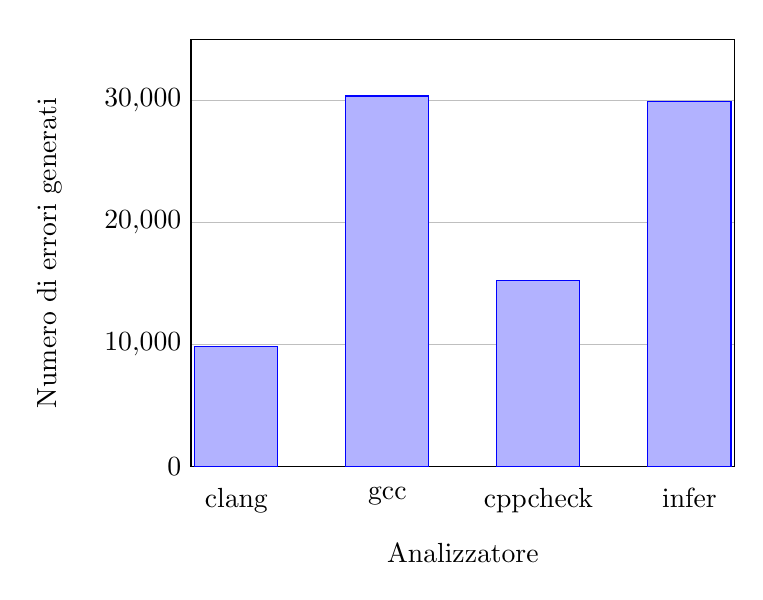
\begin{tikzpicture}
      \begin{axis}[
      width  = \textwidth * 0.7,
      height = 7cm,
      major x tick style = transparent,
      ybar=0.1pt,
      bar width=30pt,
      ymajorgrids = true,
      ylabel style={yshift=2ex},
      xlabel style={yshift=-1ex},
      xlabel=Analizzatore,
      ylabel=Numero di errori generati,
      symbolic x coords={clang,gcc,cppcheck, infer},
      xtick = data,
      scaled y ticks = false,
      ymin=0,ymax=35000,
      ytick style={draw=none},
      %extra y ticks = 100,
      %extra y tick labels={},
      %extra y tick style={grid=major,major grid style={very thick,draw=red}}
      ]
      \addplot table {
        Analizzatore Numero
        clang 9855
        gcc 30386
        cppcheck 15230
        infer 29950
      };
      \end{axis}
      \end{tikzpicture}
      \caption{Numero di errori generati da ogni analizzatore}
      \label{fig:grafo_errori_generati}
  \end{figure}


\section{Seconda fase: aggregazione dei report degli errori}
Dopo la prima fase descritta nella sezione precedente avremo come risultato quattro report di errori in file separati. Questi report si distinguono per due caratteristiche principali: la struttura del file e la nomenclatura degli errori. 
Per poter andare ad'utilizzare questi risultati, e fare quindi l'aggregazione di essi, dovremo effettuare due trasformazioni: un \textit{parsing} e una \textit{normalizzazione}.


\subsection{Parsing dei report}
Il \textit{parsing} è l'analisi di un dato in forma testuale per identificarne le sue componenti principali dove, in questo caso, sono la tipologia di errore e la sua posizione. 
Nel nostro caso è possibile eseguire il parsing tramite delle specifiche \textit{regex} che, avendo diversi formati di file, saranno diverse per ognuno degli analizzatori.
Il risultato del parsing sono quindi tanti record nella forma \record{errore, posizione}, dove la posizione indica sia il percorso del file ma sia anche la riga e la colonna dell'errore.

\subsection{Normalizzazione}
Per \textit{normalizzazione} si intende il processo di uniformare ad'un unico spazio di valori i dati forniti. Questo fase è fondamentale poiché i vari analizzatori forniscono lo stesso tipo di errore sotto nomi diversi. 
Per fare un esempio possiamo guardare la \autoref{tab:nomenclature} che riassume le diverse nomenclature per il tipo di errore 'memory leak'. 

\vskip1cm
    \noindent\setlength\tabcolsep{4pt}%
    \begin{tabularx}{\linewidth}{|l|c|*{4}{>{\RaggedRight\arraybackslash}X|}}
      \hline
      Forma normalizzata & Infer & Clang & Cppcheck & GCC \\ [0.5ex]
      \hline
      Memory leak  &  MEMORY\_LEAK  & unix.Malloc, ... & memleak, memleakOnRealloc, ... &  Wanalyzer-malloc-leak\\
      \hline
    \end{tabularx} 
    \captionof{table}{Tabella delle diverse nomenclature per l'errore 'memory leak'} \label{tab:nomenclature}
\vskip1cm

Notiamo inoltre un concetto fondamentale: analizzatori diversi producono analisi a granularità diverse. 
Si può osservare granularità maggiore, per il tipo di errore 'Memory leak', da parte di Cppcheck e Clang nella \autoref{tab:nomenclature}.
Infatti tutti e due definiscono più tipologie di errori che però, per convezione di questo progetto, vengono raggruppate in un'unica macro categoria.
Al contrario ci sono invece casi in cui un analizzatore non ha sensibilità sufficiente per distinguere fra due o più categorie di errori, in questa situazione un errore di quel tipo viene normalizzato in un errore per ogni categoria che potrebbe rappresentare, si può vedere ciò nella \autoref{tab:granularità}.
Nella eventualità quindi che Clang riferisca un errore di tipo 'unix.Malloc' dopo la fase di normalizzazione avremo due errori nella stessa posizione: uno di tipo 'Memory leak' e uno di tipo 'Use after free'. 

Per effettuare la normalizzazione è stata quindi sviluppata una tabella che associa ad'ogni forma normalizzata degli errori le forme definite dagli analizzatori usati.
Questa tabella è stata poi utilizzata come dizionario per convertire le tipologie di errori.

\begin{center}
  \begin{tabular}{|c|c|}
    \hline
    Forma normalizzata & Clang  \\
    \hline
    Memory leak  &  unix.Malloc, ... \\
    \hline
    Use after free & unix.Malloc, ... \\
    \hline
  \end{tabular}
  \captionof{table}{Tabella che mostra come un determinato errore di un analizzatore potrebbe corrispondere a più forme normalizzate} \label{tab:granularità}
\end{center} 

%vengono definiti più errori, nella stessa posizione, per ogni categoria che potrebbe rappresentare quell'errore.

\subsection{Aggregazione dei report}
Una volta definite le trasformazioni da effettuare possiamo introdurre l'effettivo argomento di questa sezione, cioè l'aggregazione dei quattro file prodotti dagli analizzatori.
Il processo di aggregazione permette di generare un unico report finale degli errori, andando a prendere soltanto quelli che sono stati individuati da almeno $n$ analizzatori. 
Modificando il parametro $n$ andremo, di conseguenza, a modificare la precisione e la dimensione del dataset nel seguente modo:
  \begin{itemize}
    \item Ponendo $n=1$ avremo la dimensione massima del dataset, in cui ogni singolo errore riportato viene mantenuto, a scapito però di un numero di falsi positivi più grande.
          Notiamo comunque, e questo vale per tutti i valori di $n$, che nel caso di duplicati ne viene sempre inserito solo uno.
    \item Ponendo $n=2$ avremo un bilanciamento fra precisione e dimensione del dataset. 
        %Infatti come è stato notato empiricamente è alquanto raro che più di due degli analizzatori individuino un specifico errore,
          %quindi con $n=2$ manterremo comunque un sufficiente numero di dati migliorandone però la precisione.
    \item Ponendo $n>2$ invece il numero di errori diventa così basso che renderebbe difficile addestrare una rete, il numero però di falsi positivi diminuisce di conseguenza.
  \end{itemize}
Si può vedere in modo più chiaro come al variare del valore di $n$ cambi il numero di errori ottenuti in \autoref{fig:grafo_aggregazione}.
Nel caso di questo lavoro sono stati utilizzati dataset sia derivanti dal porre $n=1$ sia dal porre $n=2$.

\begin{figure}
    \centering
    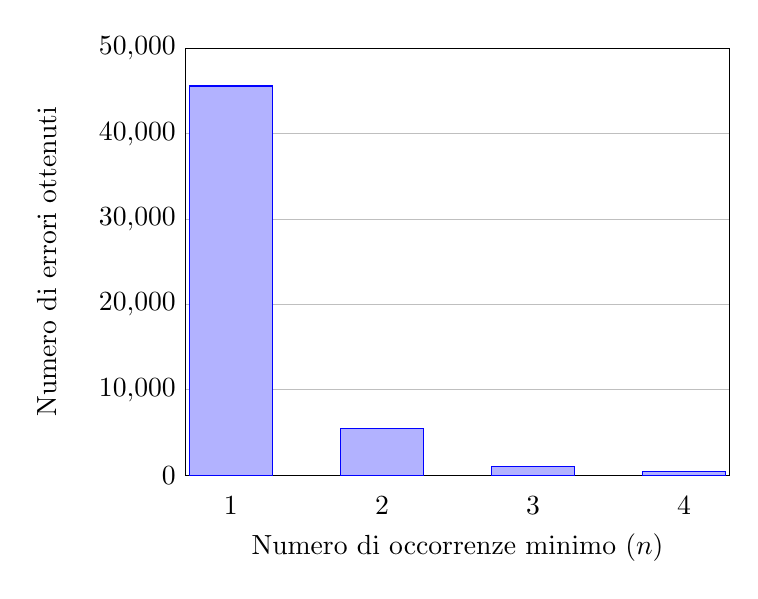
\begin{tikzpicture}
    \begin{axis}[
    width  = \textwidth * 0.7,
    height = 7cm,
    major x tick style = transparent,
    ybar=0.1pt,
    bar width=30pt,
    ymajorgrids = true,
    ylabel style={yshift=2ex},
    xlabel=Numero di occorrenze minimo ($n$),
    ylabel=Numero di errori ottenuti,
    xtick = data,
    scaled y ticks = false,
    ymin=0,ymax=50000,
    ytick style={draw=none},
    %extra y ticks = 100,
    %extra y tick labels={},
    %extra y tick style={grid=major,major grid style={very thick,draw=red}}
    ]
    \addplot table {
      N Numero 
      1 45606
      2 5423
      3 1049
      4 433
    };
    \end{axis}
    \end{tikzpicture}
    \caption{Numero di errori aggregati ottenuti in variazione del numero $n$ di occorrenze minime}
    \label{fig:grafo_aggregazione}
\end{figure}

\section{Fase due: associazione tra errore e codice}
Lo scopo di questa fase è quello di mappare la posizione di ogni singolo errore ad'un determinato \textit{code snippet}.  


%\subsection{Fase 1: utilizzo di analizzatori statici per la generazione di report di errori}

%\subsection{Fase 2: aggregazione dei report}

%\subsbusection{Conversione degli errori}

%\subsection{Fase 3: }

%\subsection{Fase 4: generazione degli Ast Context}

%\section{Statistiche finali del dataset}